\documentclass[tikz, border=5pt]{standalone}
\usepackage{xstring}
\usetikzlibrary{decorations.pathreplacing,
positioning}

\newcommand{\GetBit}[2]{%
    \edef\BitPos{#2}%
    \StrLen{#1}[\StringLen]%
    \ifnum\BitPos>\StringLen
        \edef\Bit{0}%
    \else
        \StrChar{#1}{#2}[\Bit]%
    \fi
}
\newcommand{\SetBits}[1]{%
    \foreach \i in {1,...,16} {%
            \GetBit{#1}{\i}%
            \node at (\i - 0.5, 0.5) {\LARGE \textbf{\Bit}};
        }%
}

\begin{document}

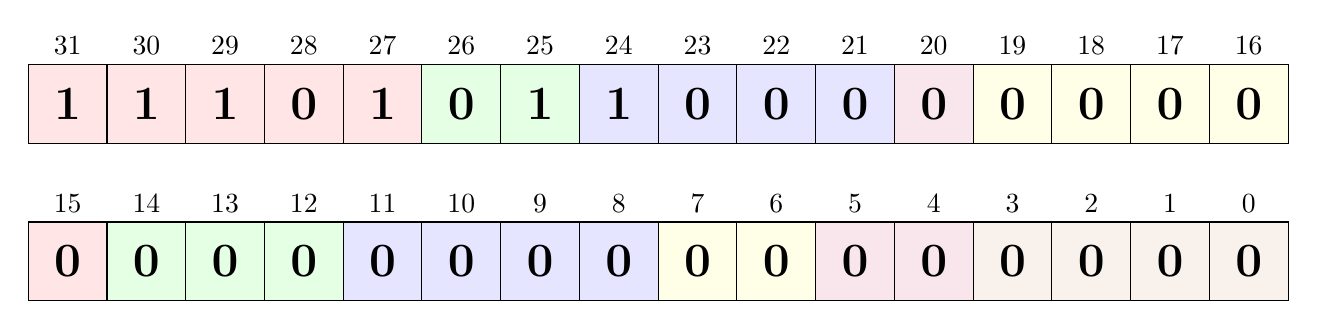
\begin{tikzpicture}

    % Colors
    \fill [red!10] (0, 0) rectangle (5, 1);
    \fill [green!10] (5, 0) rectangle (7, 1);
    \fill [blue!10] (7, 0) rectangle (11, 1);
    \fill [purple!10] (11, 0) rectangle (12, 1);
    \fill [yellow!10] (12, 0) rectangle (16, 1);

    \foreach \i in {0,...,15} {
            % Boxes
            \draw (\i, 0) rectangle (\i + 1, 1);
        }
    \foreach \i in {16,...,31} {
            % Position
            \node [above] at (31.5 - \i, 1) {\i};
        }
    \SetBits{1110101100000000}

    % Colors
    \fill [red!10] (0, -1) rectangle (1, -2);
    \fill [green!10] (1, -1) rectangle (4, -2);
    \fill [blue!10] (4, -1) rectangle (8, -2);
    \fill [yellow!10] (8, -1) rectangle (10, -2);
    \fill [purple!10] (10, -1) rectangle (12, -2);
    \fill [brown!10] (12, -1) rectangle (16, -2);

    \foreach \i in {0,...,15} {
            % Boxes
            \draw (\i, -2) rectangle (\i + 1, -1);

            % Position
            \node [above] at (15.5 - \i, -1) {\i};
        }
    \foreach \i in {1,...,16} {%
            \GetBit{0000000000000000}{\i}%
            \node at (\i - 0.5, -1.5) {\LARGE \textbf{\Bit}};
        }%

\end{tikzpicture}

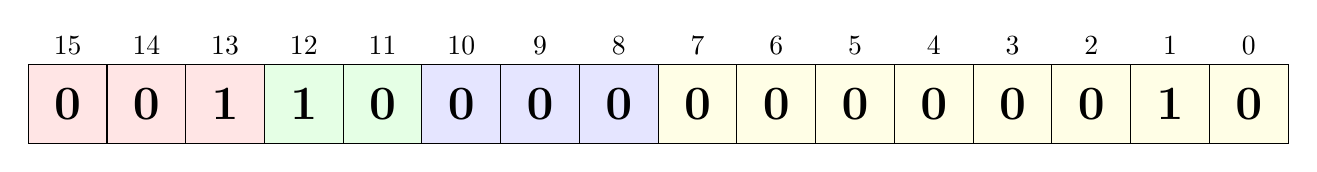
\begin{tikzpicture}

    % Colors
    \fill [red!10] (0, 0) rectangle (3, 1);
    \fill [green!10] (3, 0) rectangle (5, 1);
    \fill [blue!10] (5, 0) rectangle (8, 1);
    \fill [yellow!10] (8, 0) rectangle (16, 1);

    \foreach \i in {0,...,15} {
            % Boxes
            \draw (\i, 0) rectangle (\i + 1, 1);

            % Position
            \node [above] at (15.5 - \i, 1) {\i};
        }
    \SetBits{0011000000000010}

\end{tikzpicture}

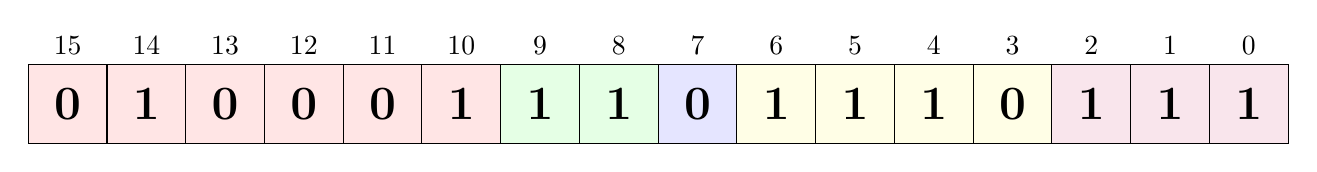
\begin{tikzpicture}

    % Colors
    \fill [red!10] (0, 0) rectangle (6, 1);
    \fill [green!10] (6, 0) rectangle (8, 1);
    \fill [blue!10] (8, 0) rectangle (9, 1);
    \fill [yellow!10] (9, 0) rectangle (13, 1);
    \fill [purple!10] (13, 0) rectangle (16, 1);

    \foreach \i in {0,...,15} {
            % Boxes
            \draw (\i, 0) rectangle (\i + 1, 1);

            % Position
            \node [above] at (15.5 - \i, 1) {\i};
        }
    \SetBits{0100011101110111}

\end{tikzpicture}

\end{document}
